\section{Transfer Learning: Representing contacts}
\label{sec:InfoForPrediction}

The input domains of $f$, $f_{qs}$ $p_{qs}$ as proposed above  adequately represent the behaviour of a specific pair of rigid bodies in a specific environment. They thus provide a well posed version of problem P1 (Action Interpolation). Given this information, however, we cannot solve problems P2 (Action Transfer) or P3 (Shape Transfer). This is because there is insufficient information: the input variables only capture {\em global} relations between objects. To properly pose transfer learning problems we must also explictly capture in the input domain all the {\em local} contact relations between the object and its surroundings. 

\begin{figure}[t]
\centerline{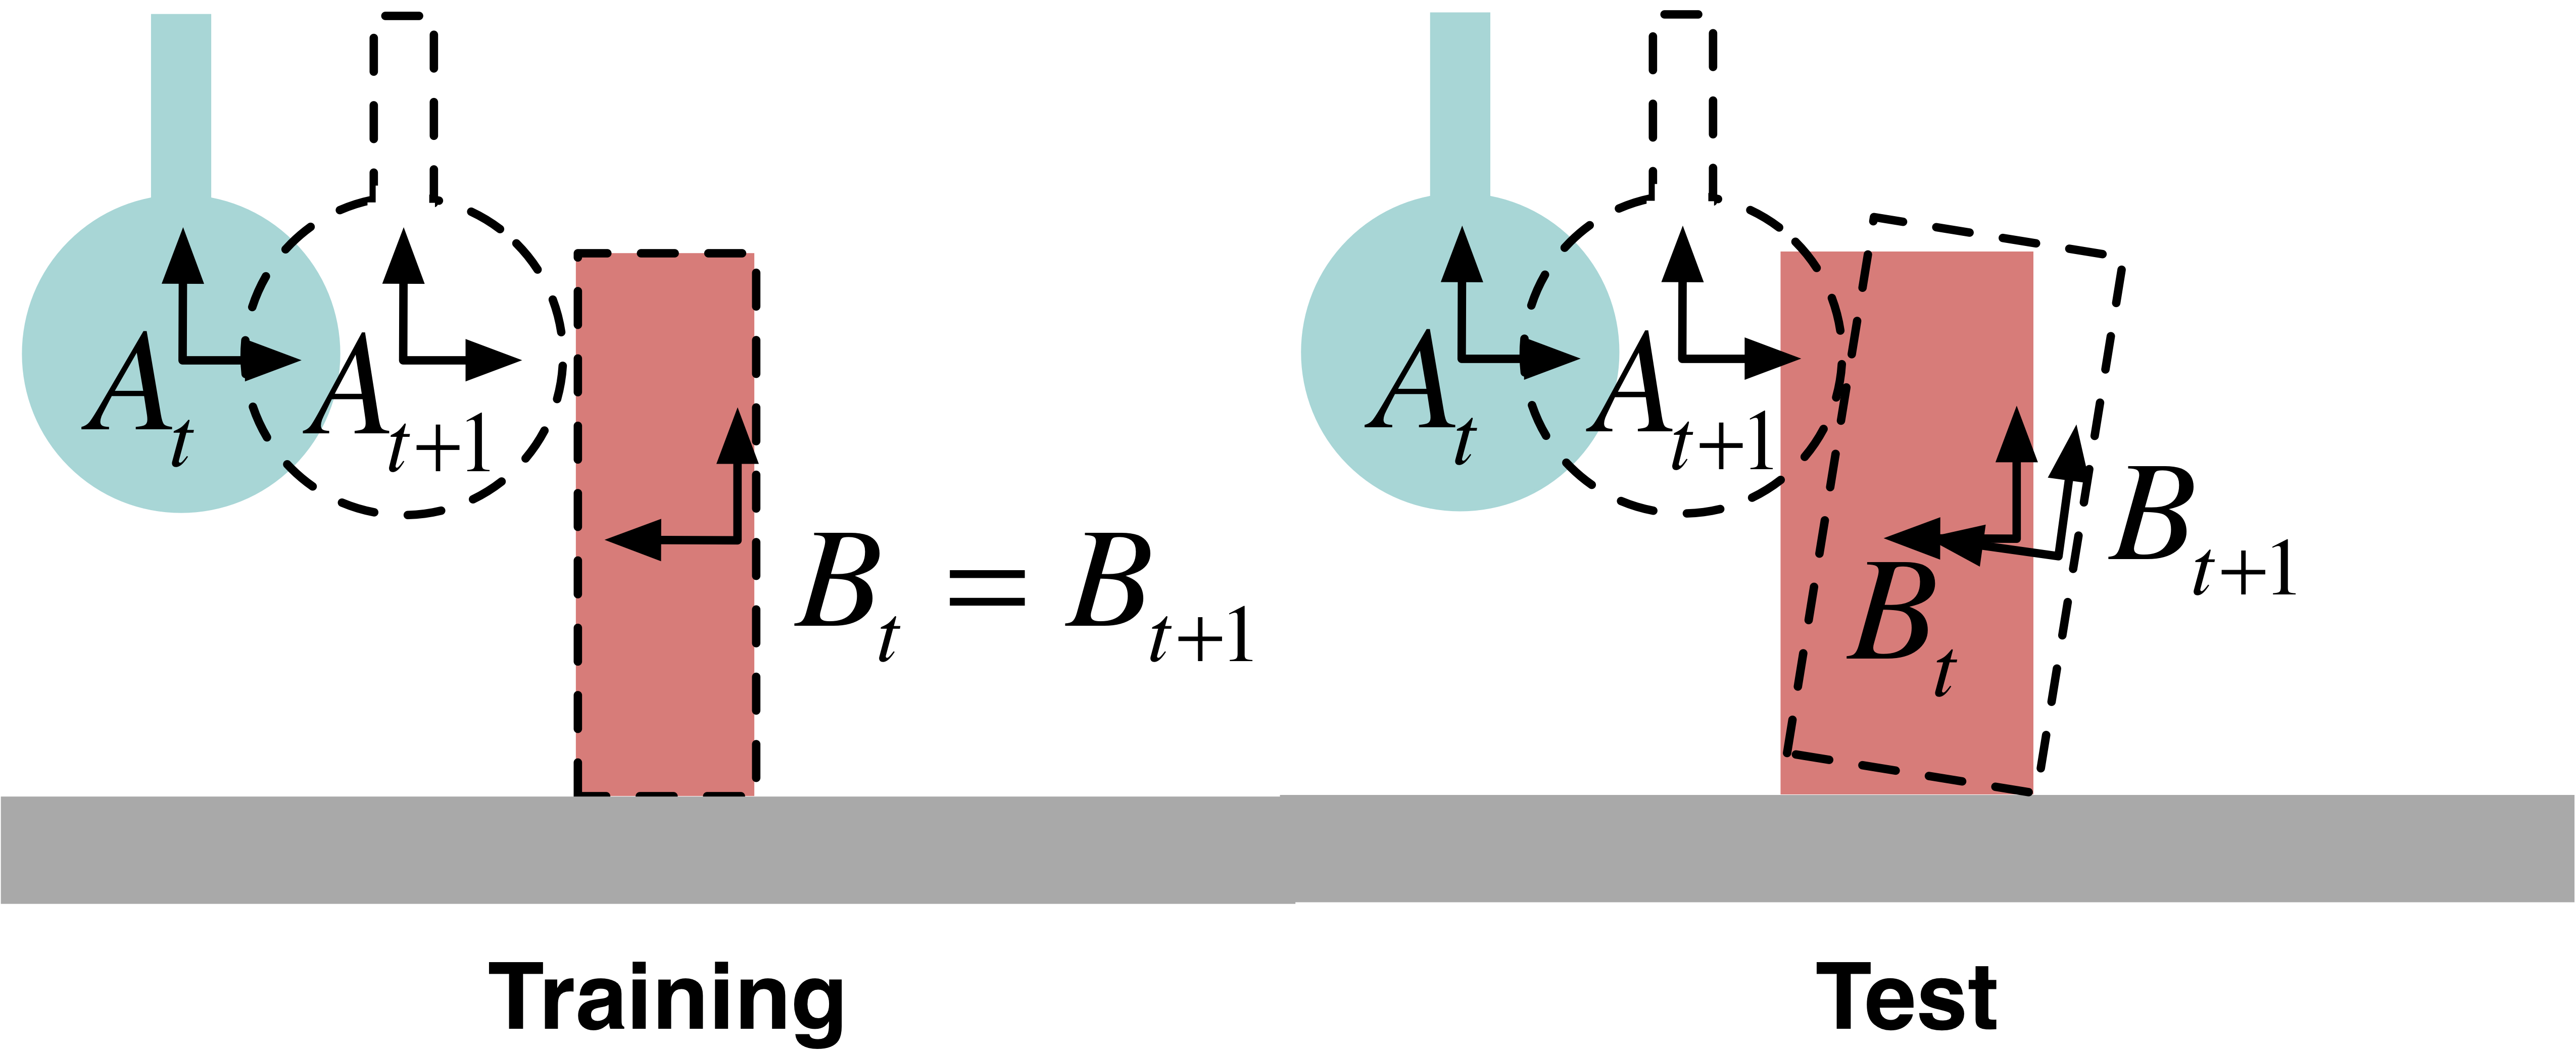
\includegraphics[width=7.5cm]{shapes-colour}}
\caption[Shapes]{Two scenes (left and right),
each with an object on a tabletop, and a finger.
Only the shape of object B differs between the scenes.
Yet when A moves to the position shown by the dashed outline at time $t+1$,
the resulting displacement of B
(represented by the transformation $T^{B_{t}, B_{t+1}}$)
will be quite different.}
\label{fig:Learning.shapes}
\end{figure}

To see why, consider a simple case of shape transfer in Figure~\ref{fig:Learning.shapes}. On the left is a training example. On the right is a test case, where the only difference is that the shape of the object has changed: it is wider. Given the same placement of the frames on object and agent, and the same finger motion, the predicted behaviour using Equation~\eqref{eq:Learning.short} must be the same as for the training example. But this is wrong. To enable the correct prediction to be transferred, additional information is needed in the input domain. Specifically, information on the contact between $A$ and $B$ is required. This can be captured by attaching additional frames to $A$ and $B$ close to their point of contact (see Figure~\ref{fig:Learning.setup2} (centre panel)).

In general an object will have multiple contacts with both the robot, and the environment. Each of these contacts provides a kinematic constraint on the motion of the object, and thus each one of these contacts should be captured as input variables. Only in this way does the predictor have sufficient information to solve transfer problems P2 and P3. Rigid body simulators employ just such contact information. 

%.  A predictor based on
%Equation~\eqref{eq:Learning.short}, and trained on the smaller object
%$B$ (Figure~\ref{fig:Learning.shapes} left scene), cannot generalise
%to the larger object (right scene). This is because the three input
%reference frames ($A_t$, $B_t$, $A_{t+1}$) in the left and right
%panels have identical poses. Thus the predictions will be identical
%even though the shapes are different. For the right panel the
%prediction will be that the finger $A$ will pass into object $B$. So,
%as posed there is insufficient information in the domain of the
%function to allow generalisation. To enable such generalisation
%information on the contact between $A$ and $B$ is required. If object
%$B$ has multiple contacts then information on all of them should be
%included. Physics simulators employ just such contact information to
%inform their predictions. 

\begin{figure*}[t]
\centerline{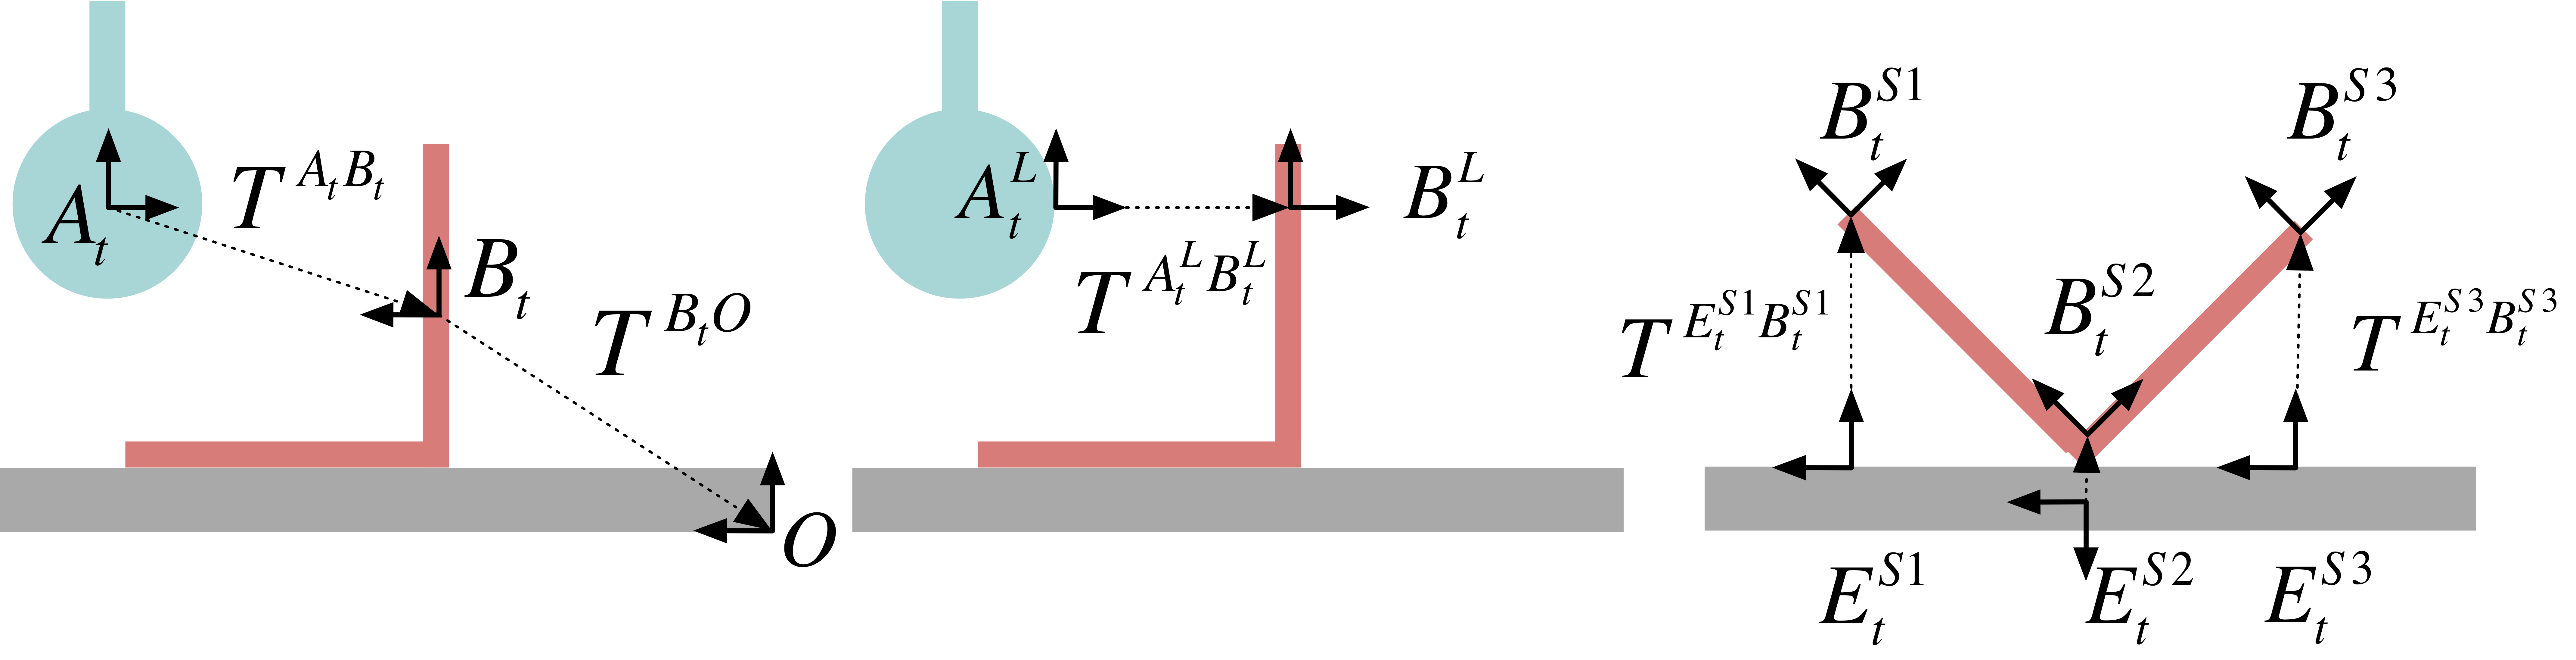
\includegraphics[width=0.75\textwidth]{information}}
\caption{Three types of information useful in prediction problems. Left: (G - global) global frames of reference for the robot, object and the world. Centre: (A - agent) local frames of reference on the robot finger and the closest point on the object. Right (E - environment) local frames of reference on the object and the closest points on surfaces in the environment.}
\label{fig:Learning.setup2}
\end{figure*}

Our approach is to use a pair of local frames to encode each contact or near contact. Each pair encodes one transformation between part of the object $B$ and another body.  To distinguish these local frame pairs from what has gone before we henceforth refer to the main frame attached to each body (as defined in Section~\ref{sec:Representations}) as the global frame for that body. 

We can formally define these local frame pairs as follows. Reconsider
the 2D projection of a robot finger with global frame $A_{t}$, an
object with global frame $B_{t}$, and the environment global frame $O$
(Figure~\ref{fig:Learning.setup2}, left panel). We now also define a pair of local frames
capturing the finger-object contact as $A^{L}_{t}$ and
$B^{L}_{t}$ (centre panel). These are spatially dynamic, i.e.\ at any time $t$ they
are located at the points of closest proximity on the finger and
object respectively.  We define the \textit{agent-object contact}
information as the transformations $T^{A^{L}_{t}, A^{L}_{t+1}}$ and
$T^{A^{L}_t, B^{L}_t}$.

We additionally define $N$ pairs of local frames $B^{Sk}_t$ and $E^{Sk}_t$ to
capture the object-environment contacts, where ($k=1 \ldots N$) (Figure~\ref{fig:Learning.setup2} right panel). We attach the $N$ frames $B^{Sk}_t$
to various parts of the object. Each has a corresponding frame in the
environment $E^{Sk}_t$.  Because they are spatially dynamic the
frames $E^{Sk}_t$ move over surfaces in the environment, as the
object moves. We define the \textit{object-environment contact}
information as the set of transformations $T^{E^{Sk}_t,B^{Sk}_t}$ for $k=1
\ldots N$. To obtain the results presented in this paper, the number and the
locations of the frames $B^{Sk}_t$ on each different object were
determined by hand. In principle this procedure could be automated,
but falls beyond the scope of the current work.

We have already motivated the need for these additional input
variables to support shape generalisation. Their utility can also be seen with respect to changes in
action. The top row of Figure~\ref{fig:ToyExample} shows a training
and a test case for problem P2 (action transfer). The prediction of the test push trajectory requires some encoding of the kinematic constraint
imposed by the contact between the base of the L-shaped flap and the
table. This constraint exists in the training push, but is not
significant since the flap can rotate around its corner, unconstrained
by the base.

\begin{figure}[b]
\centerline{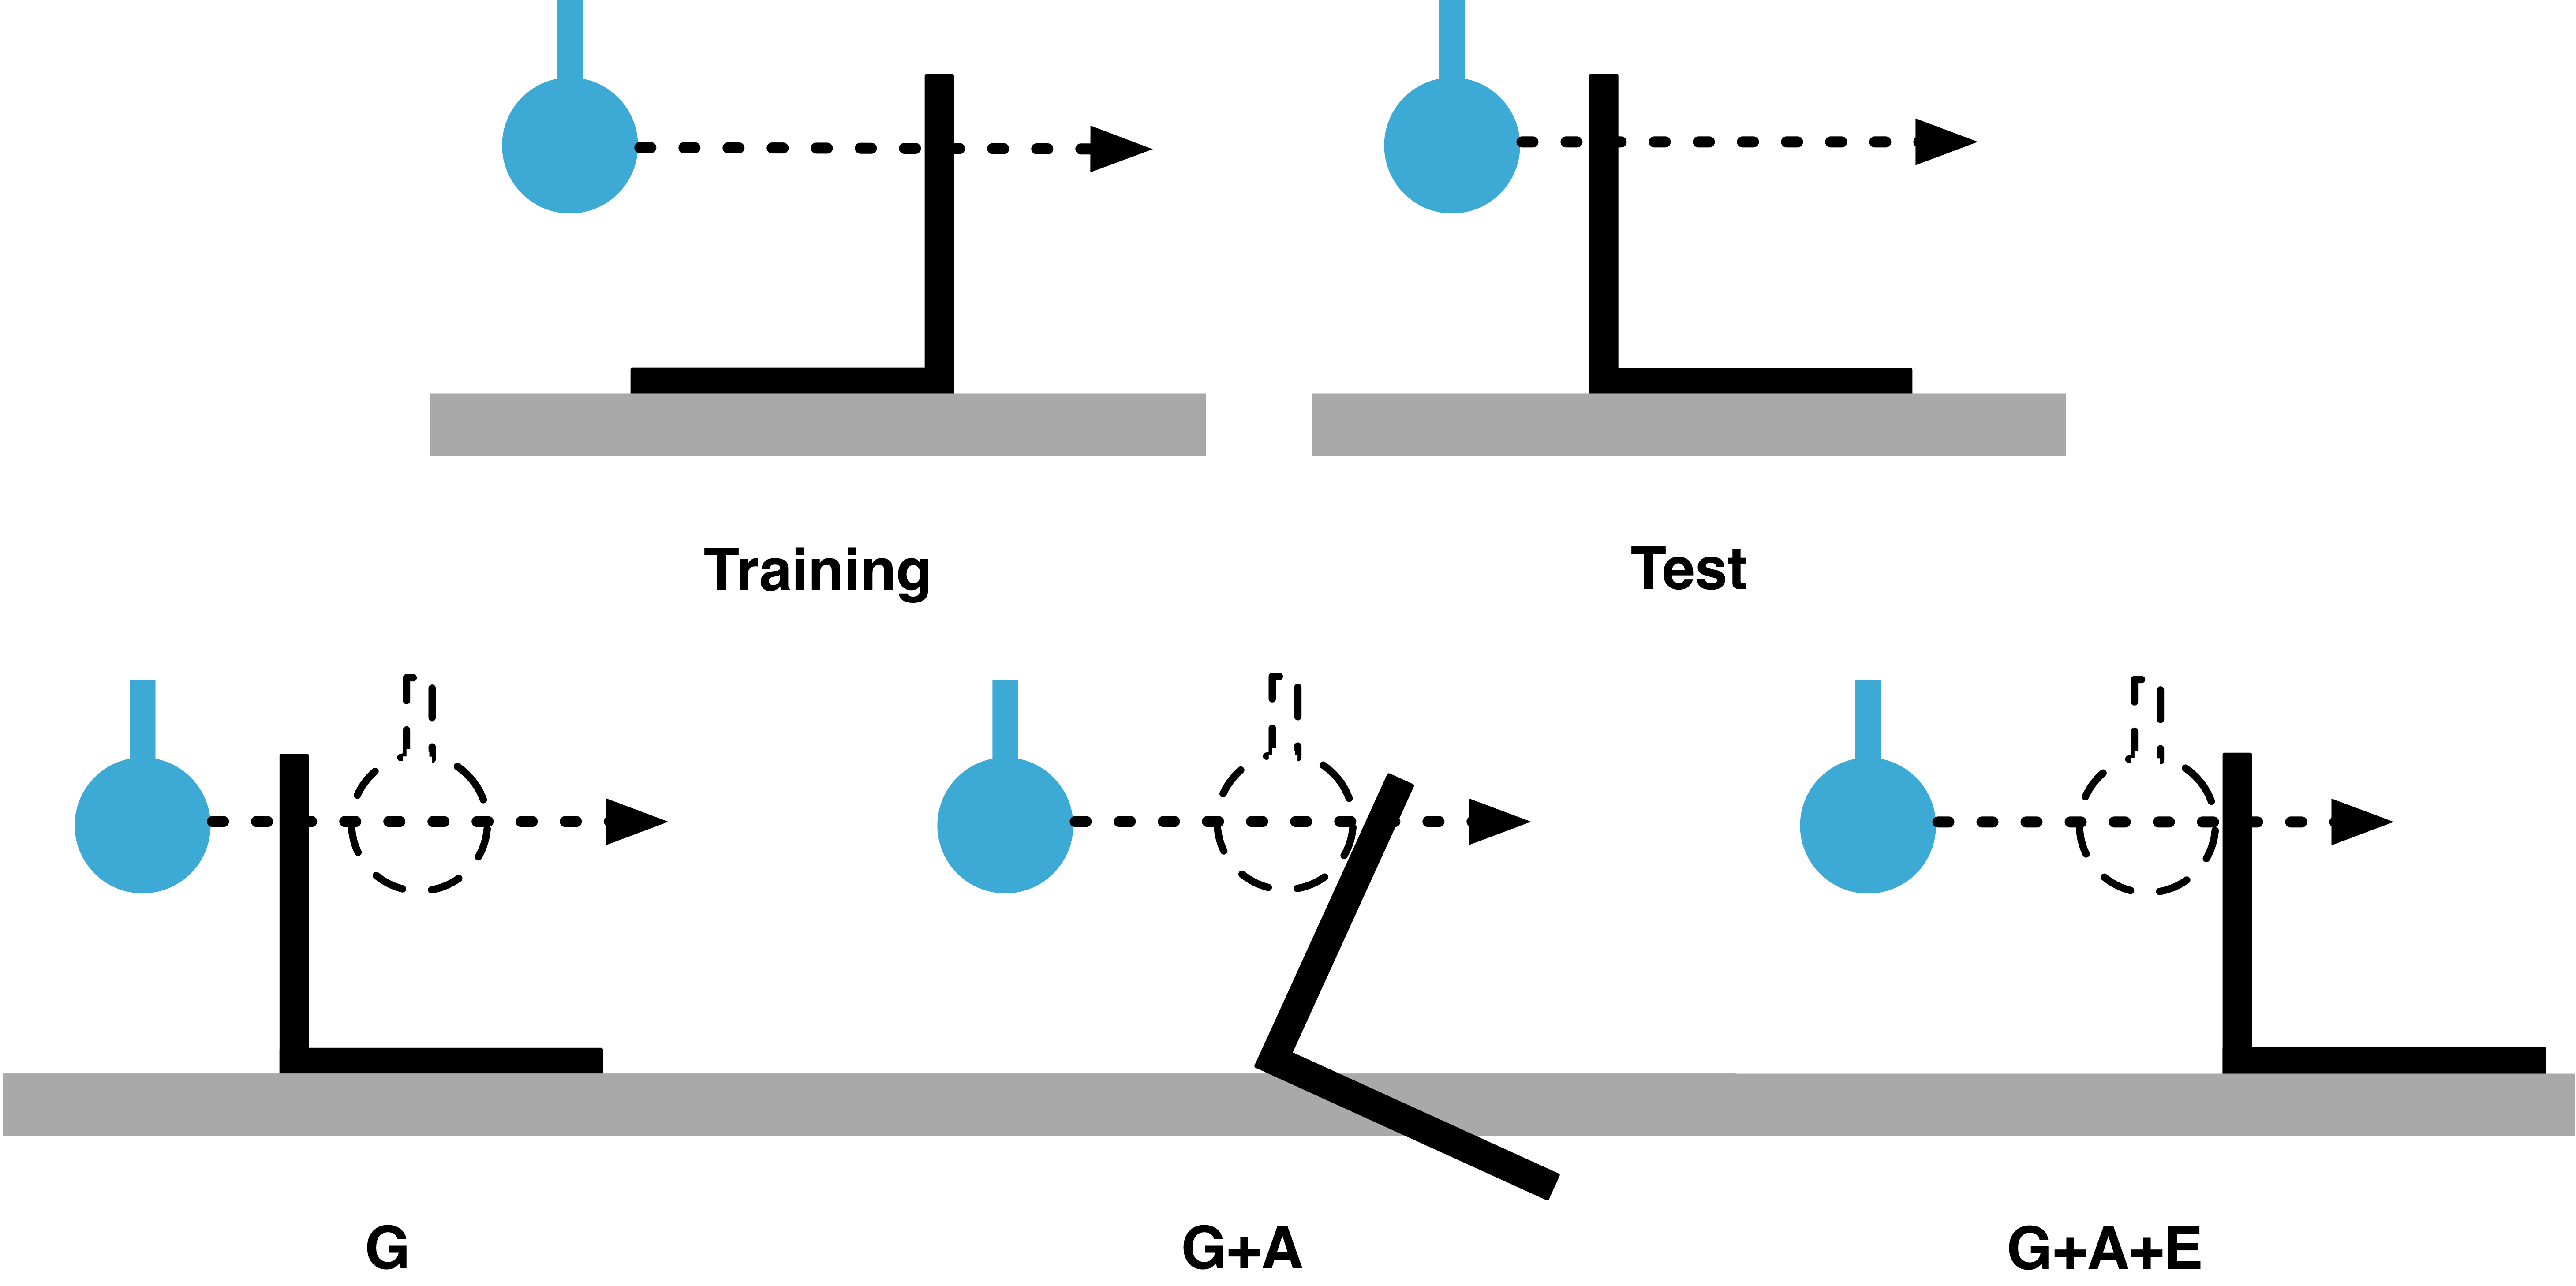
\includegraphics[width=0.8\columnwidth]{BackPushToyExample}}
\caption[ToyExample]{Schematic diagram (2D projection of 3D scene)
in which an object (of L-shaped cross-section) on a supporting surface
is pushed by a robotic finger. 
Various predictors are trained solely on forward pushes (top left), but tested on backwards pushes (top right). The top panels show the push trajectory for the training and test phases, whereas the bottom panels show the outputs from three types of predictor (G, G+A and G+A+E) in the test phase.}
\label{fig:ToyExample}
\end{figure}

We can now consider the effects that different amounts of information
might have on generalised predictions. A predictor endowed only with
information based on the global frames for each body we refer to as
having global information (G). We can add agent-object contact
information to this (G+A), and in turn we can add object-environment
contact information (G+A+E). Now consider the possible predictions for
the test case (Figure~\ref{fig:ToyExample} bottom row). A predictor
using G will predict that the object will not move, because it has no
nearby experience to suggest otherwise. A predictor using G+A has
information from the training case that the object surface will move
with the finger, so that the finger will not pass through it, but is
also capable of predicting that the object rotates about the corner
and into the table since it doesn't model the object-environment
contact. A predictor using G+A+E will have information about the
effect of the contact between the base of the flap and the table and
so should avoid predicting a rotation into the table.

One point is critical here: the above analysis only concerns what the
information allows, it depends on the ability of the learner to
utilise it.  To test this we must incorporate the information into
each learning framework. We can simply extend the regression and density
estimation frameworks to achieve this. For regression one way to
incorporate the extra information $A^{L}_{t}$,$B^{L}_{t}$ and
$E^{Sk}_t$\hspace{-6pt}, $B^{Sk}_t$, provided by the agent and
environment contacts, is simply to enlarge the domain of function~$f$
in Equation~\eqref{eq:Learning.short}, that is:
\begin{multline}
f'_{qs}: T^{A_t, B_t}, T^{B_t, O}, T^{A_{t}, A_{t+1}}, T^{A^{L}_t, B^{L}_t}\{, T^{E^{Sk}_t,B^{Sk}_t}\}_{k=1 \ldots N} \\ 
\longrightarrow T^{B_{t}, B_{t+1}}
\label{eq:Learning.augmented}
\end{multline}

\noindent Unfortunately, because the dimensionality of the domain of $f'_{qs}$ grows with the number of environment contacts $N$,
the difficulty of learning the mapping $f'_{qs}$ rapidly increases
as more environment contacts are added.


The conditional probability density (CPD) $p_{qs}$ over possible object motions $T^{B_{t}, B_{t+1}}$~\cite{kopicki_prediction_2009} is augmented as follows:
\begin{multline}
p_{qs}(T^{B_{t}, B_{t+1}} | T^{A_t, B_t}, T^{B_t, O}, T^{A_{t}, A_{t+1}}, T^{A^{L}_t, B^{L}_t}\\
\{, T^{E^{Sk}_t,B^{Sk}_t}\}_{k=1 \ldots N})
\label{eq:Learning.density}
\end{multline}

Again the dimensionality of the conditioning variables makes density
estimation hard as the number of contacts grows. One way round this in the density estimation case is to factorize the density in a way that
reflects the contact structure. We consider this in the next section. 